
\section{Implementierung des Mocks}
\label{sec:impl}
Der Mock wurde unter Einsatz des Frameworks \emph{OrbTK} implementiert. Da die prozedurale Generierung, und damit die Variabilität, erst in späteren Schritten entwickelt wird, wurde in diesem Schritt JADX mit so wenigen Veränderungen wie möglich abgebildet. In diesem Abschnitt sollen das Ziel des Mocks und die Vor- und Nachteile der Entwicklung mit OrbTK erläutert werden, bevor die Eigenschaften und Limitierungen der Implementierung beschrieben werden.

\subsection{Ziel des Mocks}
\label{subsec:goal_mock}
Das Ziel hinter der Entwicklung dieses Mocks ist es, eine Datenquelle zu schaffen, die zum Training von Autoencodern verwendet werden kann. Diese Datenquelle soll aus validen Abbildern von \gls{gui}-Oberflächen bestehen und sich an der Anwendung JADX orientieren. Dabei geht es vorwiegend darum, real aussehende \glspl{gui} zu erstellen um herauszufinden, ob und wie \gls{gui}-Oberflächen von Autoencodern enkodiert werden können. Eine exakte Nachbildung von JADX ist daher nicht nötig und aus Gründen des Zeitaufwandes auch nicht sinnvoll. Es wird allein deshalb zu Abweichungen kommen, da OrbTK sich nicht an der Windows-Designsprache oder dem Design von JADX orientiert.

Eine sekundär zu beantwortende Frage ist, wie gut die Autoencoder noch mit der realen \gls{gui} von JADX funktionieren. In Kapitel \ref{cha:autoencoder} wird daher untersucht, inwiefern die Abweichungen zwischen Mock und realer \gls{gui} einen Effekt auf die Ergebnisse der Autoencoder haben.

Die Implementierung dieses Mocks wird in dieser Arbeit außerdem so beschränkt, dass nur \gls{gui}-Elemente, die Teil von JADX sind, umgesetzt werden. Funktionen, die durch das Betriebssystem bereitgestellt werden, sind ausgenommen. Hiervon sind Dialoge zum Öffnen von Dateien sowie zur Auswahl von Schriftarten betroffen.

\subsection{OrbTK}
Mit OrbTK war es möglich, alle wichtigen \gls{gui}-Elemente in zufriedenstellender Qualität umzusetzen. Das Framework setzt auf Widgets, die den Kern darstellen und jeweils einem \gls{gui}-Element entsprechen. Widgets können komponiert werden, um neue Widgets zu kreieren. Das Aussehen kann über das Setzen von Parametern per Builder-Entwurfsmuster verändert werden, das OrbTK umsetzt \cite{RedoxosOrbtk2015}. Alternativ können Theme-Dateien verändert werden, in denen Stile definiert werden können, die während des Startens der Applikation geladen werden. Für die Entwicklung im Rahmen dieser Masterarbeit wurden die Widgets in Komponenten und Elemente aufgeteilt. Komponenten stellen größere Bausteine dar, die eine eigene Funktion darstellen oder mindestens aus mehreren Elementen zusammengesetzt sind. Elemente sind grundlegende Bausteine der \gls{gui}, wie Buttons, Eingabefelder oder Beschriftungen.

Der größte Nachteil von OrbTK ist das Layout-System, das nicht immer fehlerfrei arbeitet. Während der Implementierung kam es häufiger vor, dass \gls{gui}-Elemente ihre Position verändern, ohne, dass der Grund für diese Veränderung ersichtlich war. Darüber hinaus kann es vorkommen, dass das Setzen von Parametern keinen Effekt hat. Beispielsweise haben die Parameter, um die Höhe und Breite von \gls{gui}-Elementen zu setzen, teilweise keine Funktion, wenn sich ein Element innerhalb eines Eltern-Elements befindet. Dieses Verhalten trat scheinbar zufällig auf und war nicht reproduzierbar.

% Kind-Elemente scheinen sich oft ihrem Eltern-Element in der Größe anzupassen. In diesen Fällen sind die einzigen Möglichkeiten, die Größe von Kind-Elementen anzupassen, Grid-Layouts und Margins, welche jedoch wieder Probleme hinsichtlich responsivem Verhalten mit sich bringen und nur beschränkt konfigurierbar sind. Die Komplexität des Layouts ist insgesamt nicht mit der Komplexität der Stylesheet-Sprache CSS vergleichbar.

Außerdem ist es nicht möglich Parameter, die in speziellen Theme-Dateien gespeichert sind, im Anschluss programmatisch zu überschreiben. Theme-Dateien bieten die Möglichkeit, wiederverwendbare Stile für einzelne \gls{gui}-Elemente zu definieren. Wenn solche Parameter einmal gesetzt wurden, können sie im Rust-Quelltext nicht mehr überschrieben werden. Der in Rust gesetzte Parameter wird ignoriert. Neben dem fehlenden Fehlerfeedback ist das problematisch, da so ein neuer Style in der Theme-Datei für ein einzelnes \gls{gui}-Element definiert werden muss und die Theme-Datei dadurch unnötig fragmentiert. Eine andere Möglichkeit ist, die Parameter im Rust-Quelltext und nicht mehr in der Theme-Datei zu setzen. Dieses Vorgehen führt jedoch zu dupliziertem Quelltext.

Bei OrbTK ist es des Weiteren schwer, Fehler zu identifizieren, da bestimmte Parameter nicht typsicher sind. Die horizontale und vertikale Ausrichtung von Elementen oder das Layout von Grids werden beispielsweise nur als String angegeben. Die Höhe und Breite von Elementen wird als Gleitkommazahl erwartet. Wird stattdessen eine Ganzzahl übergeben, ignoriert OrbTK diesen Wert und gibt keine Fehlermeldung aus. Wenn solche Probleme auftreten und das Aussehen der \gls{gui} nicht mit dem gewünschten Layout übereinstimmt, gibt es kaum Möglichkeiten zu debuggen. Rust-Debugger helfen hier oft nicht weiter, da das entsprechende Verhalten sehr tief in OrbTK auftritt und nicht im Quelltext des Benutzers. Da zusätzlich meist keine Dokumentation vorhanden ist, war so nur \emph{Trial and Error} als Lösungsstrategie möglich.

\subsection{Eigenschaften}

Um JADX abzubilden, wurden die wichtigsten Ansichten von JADX im Mock nachgebaut. Hierzu zählen die Hauptansicht, die Ansicht für die Einstellungen, die Ansichten für Text- und Klassensuche und die Ansicht für die Suche nach Benutzung von Java-Klassen, Attributen und Parametern. Daneben existieren Ansichten für Lognachrichten, das Umbenennen von einzelnen Paketen und Java-Entitäten sowie die About-Ansicht. Alle Ansichten werden entsprechend in neuen Fenstern geöffnet und sind, bis auf die Ansicht für Lognachrichten, im Mock vorhanden. Einige davon werden in den Abb. \ref{fig:mock_comparison} bis \ref{fig:mock_search_comparison} gegenübergestellt.

Ein besonderer Fokus lag darauf, Gruppierungen von \gls{gui}-Elementen möglichst detailgetreu abzubilden. Container, die solche Elemente beinhalten, und Abgrenzungen, welche diese separieren, wurden entsprechend nachgebaut. Die Buttons, Menüs, Eingabefelder etc. wurden entsprechend in ihrem Aussehen angeglichen und, wenn nicht verfügbar, nachgebaut. Um Buttons und \gls{gui}-Elemente zu erstellen wurden die in JADX eingebetteten Bilder und Icons wiederverwendet.

% Während der Entwicklung wurden in diesem Schritt auch schon Logiken umgesetzt, um Daten zur Laufzeit hinzuzufügen und zu verändern. Die \gls{gui} wurde somit nicht hart kodiert. Durch diese Maßnahmen kann ein Generator, der gültige Instanzen der \gls{gui} zufällig erzeugen soll, leichter geschrieben werden. Des Weiteren wurde auf eine möglichst responsive Umsetzung geachtet, um die Umsetzung der prozeduralen Generierung zu vereinfachen.


\begin{figure}[p]
    \centering
    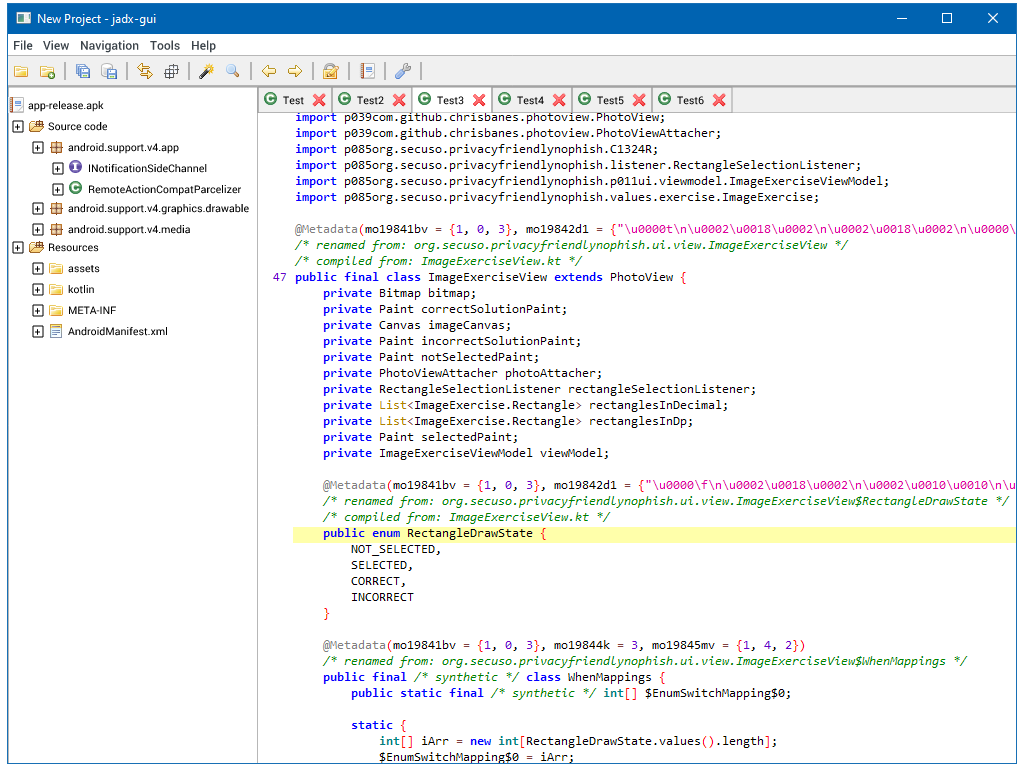
\includegraphics[height=.45\textheight]{bilder/jadx_mock_main.png}
    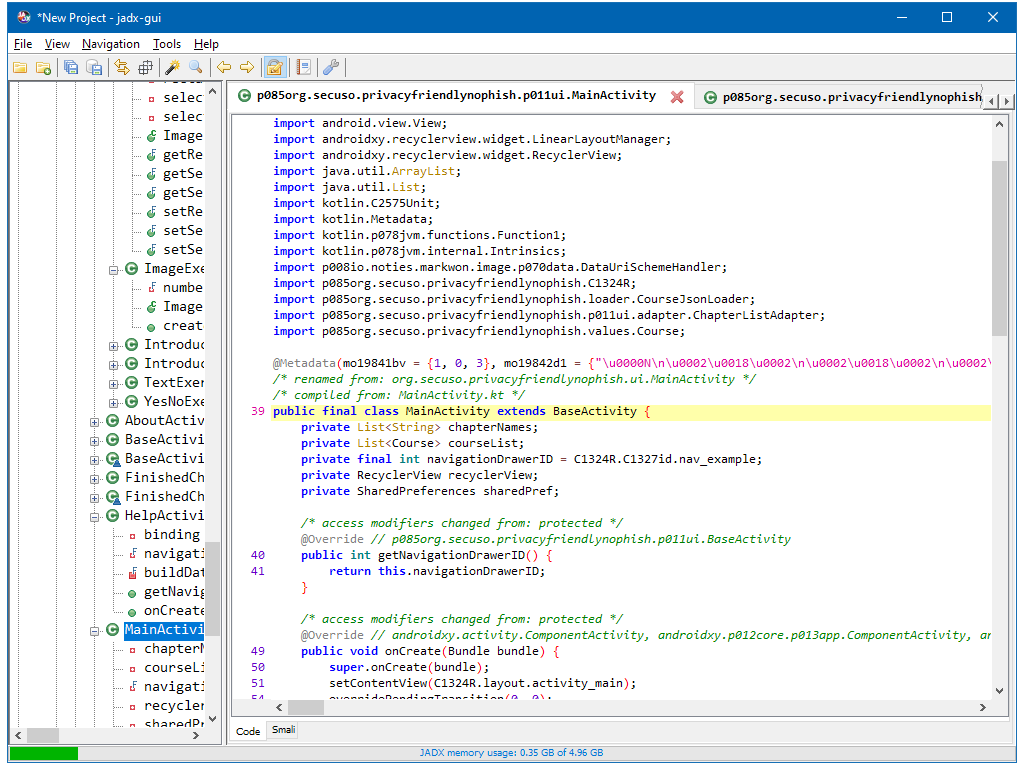
\includegraphics[height=.45\textheight]{bilder/jadx_main.png}
    \caption{Vergleich Hauptansicht: Mock (oben) und JADX (unten)}
    \label{fig:mock_comparison}
\end{figure}

\begin{figure}[p]
    \centering
    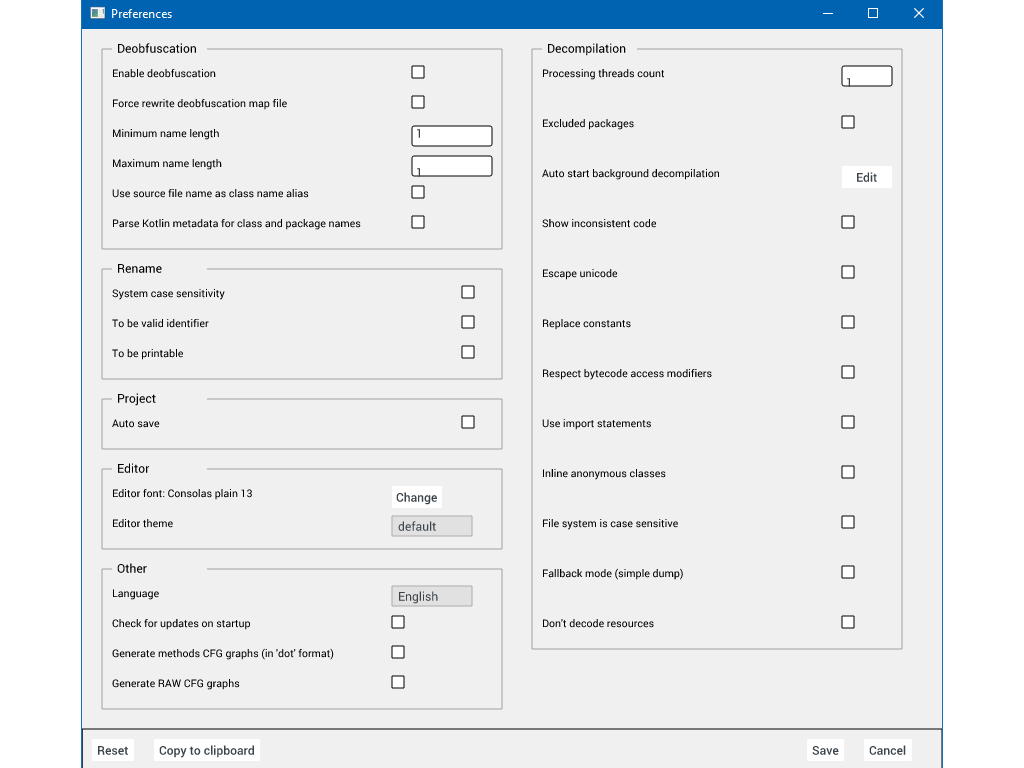
\includegraphics[height=.45\textheight]{bilder/jadx_mock_settings.png}
    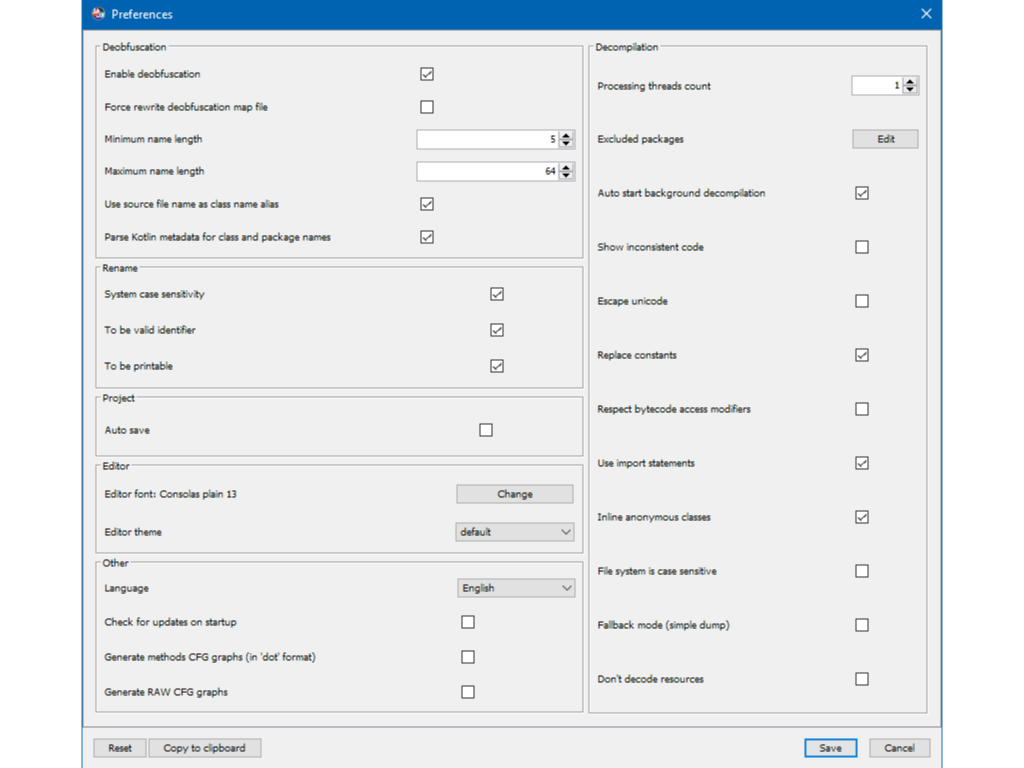
\includegraphics[height=.45\textheight]{bilder/jadx_settings.png}
    \caption{Vergleich Einstellungen: Mock (oben) und JADX (unten)}
    \label{fig:mock_settings_comparison}
\end{figure}

\begin{figure}[p]
    \centering
    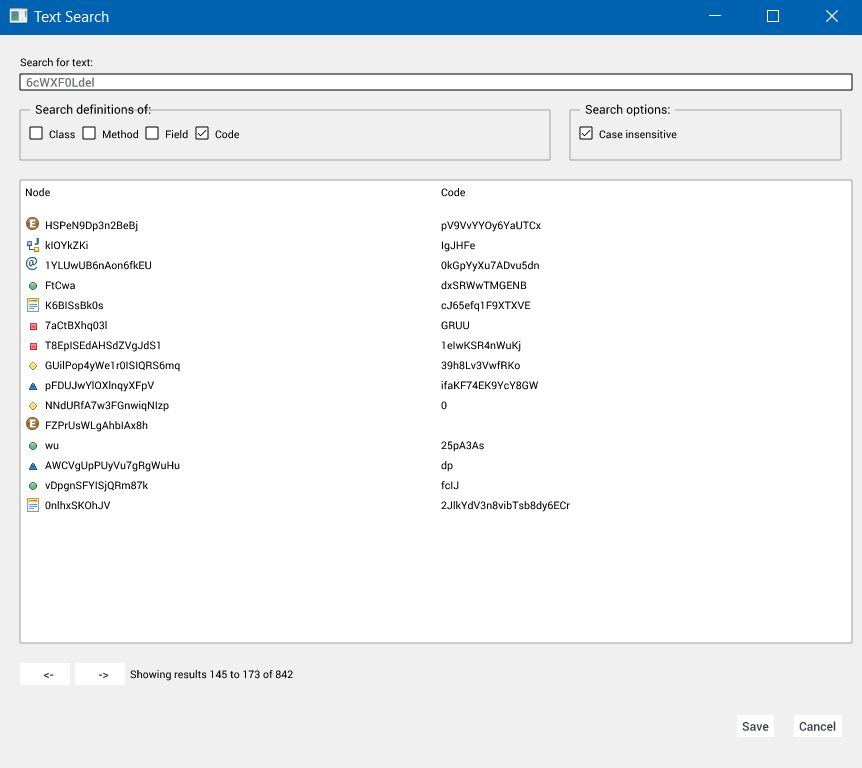
\includegraphics[height=.45\textheight]{bilder/jadx_mock_search.png}
    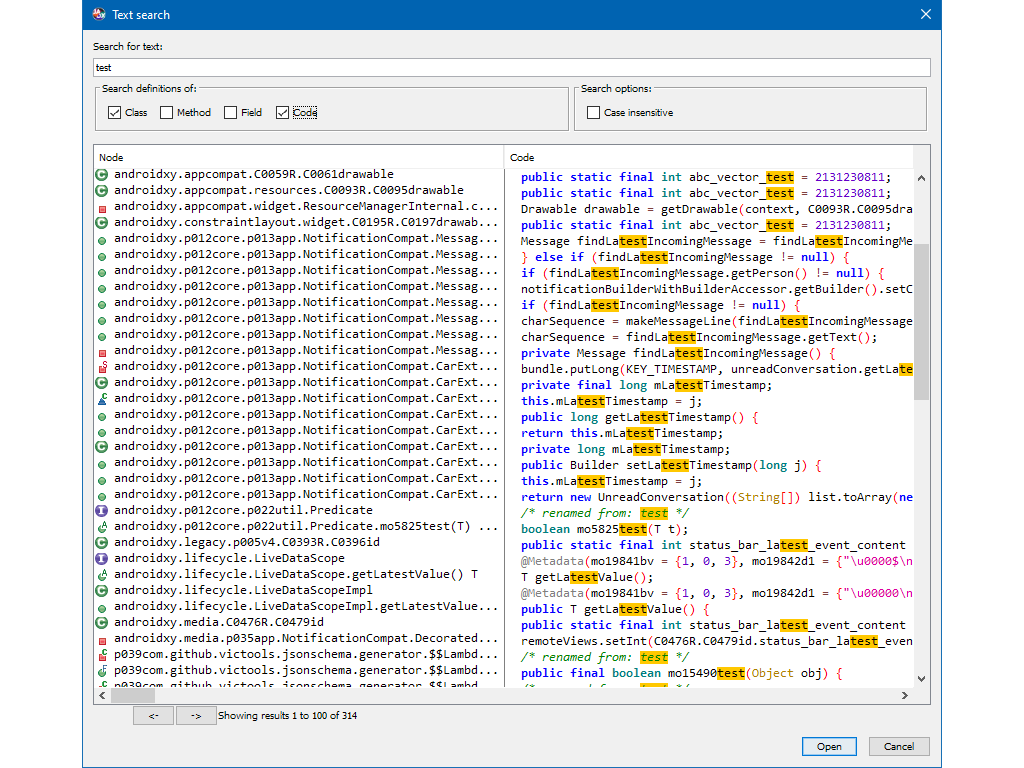
\includegraphics[height=.45\textheight]{bilder/jadx_search.png}
    \caption{Vergleich Text- / Klassensuche: Mock (oben) und JADX (unten)}
    \label{fig:mock_search_comparison}
\end{figure}





\subsection{Limitierungen}
\label{sec:mock_limitations}



Die Limitierungen der Umsetzung ergeben sich zunächst aus den Limitierungen und Fehlern von OrbTK, insbesondere der Rendering-Funktionen. Die meisten Elemente aus JADX sind nicht in OrbTK vorhanden, weshalb sie nachgebaut werden mussten. Das Design der JADX-Applikation, das sich an Windows-Designsprachen orientiert, konnte nicht immer exakt umgesetzt werden, sodass sich kleinere Abweichungen ergeben. OrbTK bietet die Möglichkeit Rahmen um Container innerhalb der Applikation zu ziehen, ähnlich wie sie in JADX oft verwendet werden. Selbst ein Rahmen der Breite \texttt{1}, die kleinste darstellbare Breite, erscheint dicker, als die innerhalb JADX verwendeten Rahmen. Weitere Features wie Schattierungseffekte oder gepunktete Linien (beispielsweise Verbindungslinien des Projekt-Baums in der Hauptansicht von JADX) sind nicht in OrbTK verfügbar.

\todo{Sind diese Abweichungein ein Problem? --> Später in der Arbeit genauer erörtern und Testset aus richtiger JADX-Applikation verwenden}

Die Funktionalität, um mehrere Fenster zu öffnen, ist in OrbTK grundsätzlich vorhanden. JADX verwendet dies beispielsweise um eine Volltext- oder Klassensuche durchzuführen. Das Öffnen zusätzlicher Fenstern ist in OrbTK jedoch aktuell noch sehr fehlerhaft. Wenn die Fenstergröße nach dem Öffnen beispielsweise durch den Mauszeiger verändert wird, wird der Inhalt des Fensters schwarz. Für diese Masterarbeit ist dieser Umstand jedoch kein Problem, da Fenster nur einmal gerendert werden, bevor sie als Bild gespeichert werden. Dadurch finden nach dem initialen Rendering keine Veränderungen mehr statt. Es existieren ähnliche Probleme bezüglich der Ausführung von Aktionen durch den Benutzer. In zusätzlichen Fenstern werden Mausklicks oft nicht registriert, sodass diese mehrfach durchgeführt werden müssen. Auch diese Fehler sind für diesen Anwendungsfall nicht relevant, da für die Experimente im Rahmen dieser Arbeit keine Aktionen mit der Maus durchgeführt werden. Alle Felder, die innerhalb von JADX erreichbar sind, werden vorausgefüllt.

\begin{figure}[h]
    \centering
    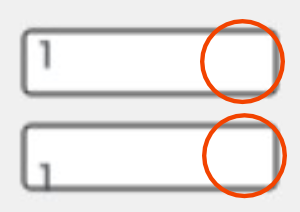
\includegraphics[scale=0.5]{bilder/NumericBoxPfeile.png}
    \caption{\texttt{NumericBox} mit fehlenden Buttons zum In- und Dekrementieren}
    \label{fig:numeric_box}
\end{figure}


In JADX werden darüber hinaus manche \gls{gui}-Elemente, wenn sie in einem zusätzlichen Fenster geöffnet werden, nicht angezeigt. Innerhalb der Box zur Eingabe numerischer Werte (\texttt{NumericBox}) werden die Buttons, durch welche der Wert in- oder dekrementiert werden kann, nicht angezeigt. Dies wird in Abb.~\ref{fig:numeric_box} dargestellt.
Weitere Unterschiede zwischen JADX und der Umsetzung des Mocks ergeben sich aus den Limitierungen von OrbTK in Verbindung mit der Umsetzungszeit. Wie in Abschnitt \ref{subsec:goal_mock} beschrieben ist, war es auch kein Ziel hinter der Entwicklung, JADX zu 100\% abzubilden. Viele Effekte, wie Schattierungen oder Verbindungslinien im Strukturbaum in der Hauptübersicht in Abb.~\ref{fig:mock_comparison}, sind so nicht in OrbTK vorhanden und nur mit unverhältnismäßigem Aufwand nachzubauen. Teilweise wurden auch \gls{gui}-Elemente implementiert, deren Design dem von JADX ähnlich ist, die jedoch keine Funktion haben. Ein Beispiel hierfür ist die Tab-Navigation über dem Editor. Die einzelnen Tabs sind nicht mit Daten hinterlegt, sodass bei einem Klick auf einen Tab nichts passiert. Da nur Abbilder der \gls{gui} verwendet werden und keine Aktionen ausgeführt werden, ist dies jedoch auch nicht notwendig. Features von JADX, wie die Speicherverbrauchsanzeige am unteren Fensterrand oder die kleinere Tabnavigation (\glqq Code\grqq\ und \glqq Smali\grqq ), wurden nicht umgesetzt.


% \begin{itemize}
%     \item Was wird für eine GUI benötigt?
%     \begin{itemize}
%         \item \textit{Welche Menüs?}
%         \item \textit{Welche Buttons? Wo platzieren?}
%         \item \textit{Styling?}
%     \end{itemize}
% \end{itemize}
